\chapter{Experimental Setup}
\label{sec:setup}

% Source notes: Project/docs/thesis_notes.md; checkpoint_2026-10-10.md; configs Project/GroundOne/configs/train_0.5b.yaml,
% train_3b.yaml; queues Project/jobs/queue_night3.txt, queue_day4.txt, queue_night5.txt, queue_day5.txt, queue_night6.txt.

This chapter presents the models that were trained, the systems they are compared with, the metrics, the statistical
protocol and the way time and energy are measured. All experiments run on a single machine: a MacBook Pro with an Apple
M4 chip and 16\,GB of unified memory, with a 10-core CPU, a 10-core GPU and a memory bandwidth of
120\,GB/s~\cite{apple2024m4specs}. Every result therefore reflects what a verifier can do on the same device on which a
local assistant runs. All the baselines, including the encoders and the two general-purpose decision models, also run
on this laptop, and no result depends on a remote service.

\section{Models}
\label{sec:setup-models}

Both GroundOne models start from the instruction-tuned version of Qwen2.5~\cite{qwen2024qwen25}, converted to MLX with
8-bit weights, and both are trained with the procedure described in Section~\ref{sec:method-training}. The two models
differ in only three respects: their size, the number of training answers and the composition of the micro-batches,
which depends on the available memory.

The 0.5B model is trained on the whole training set of 13{,}203 answers. One epoch of 802 optimiser steps took 5.5 hours
of wall-clock time\footnote{\emph{Wall-clock} time is the real time elapsed from the start to the end of an operation,
as a clock would measure it, waiting included. It differs from CPU time, which counts only the time in which the
processor is actually working.} and used at most 2.6\,GB of memory; every 150 steps the model was evaluated on the whole
dev set. The 3B model, by contrast, is about six times slower per token. It is therefore trained over one night on a
random subset of 6{,}500 answers, corresponding to about 45{,}000 decisions: 403 steps in 12.25 hours, with a peak of
5.9\,GB. A complete evaluation on the dev set would take about an hour, so the 3B is evaluated every 80 steps on a fixed
subset of 200 answers. In both cases the checkpoint with the highest three-way balanced accuracy on the dev set is kept
and then calibrated as described in Section~\ref{sec:method-calibration}; for the 3B this is step 320.

The seed determines the initialisation of the adapters and the order of the batches, and the outcome of fine-tuning is
known to vary with both factors~\cite{dodge2020finetuning}. To estimate how much the results depend on the seed, the
0.5B procedure is therefore repeated with a second seed. This second run was completed and is evaluated on all three
test sets exactly like the first. A further run with a third seed, instead, collapsed early to a constant prediction and
was stopped at about 60\,\% of the epoch. Being incomplete, it is excluded from the tables, and it is discussed in
Section~\ref{sec:results-seeds}.

\section{Baselines}
\label{sec:setup-baselines}

The baselines serve to isolate the origin of any advantage of GroundOne, and each of them answers a specific question.
Figure~\ref{fig:setup-baselines} summarises what each baseline changes with respect to GroundOne.

\begin{figure}[htbp]
\centering
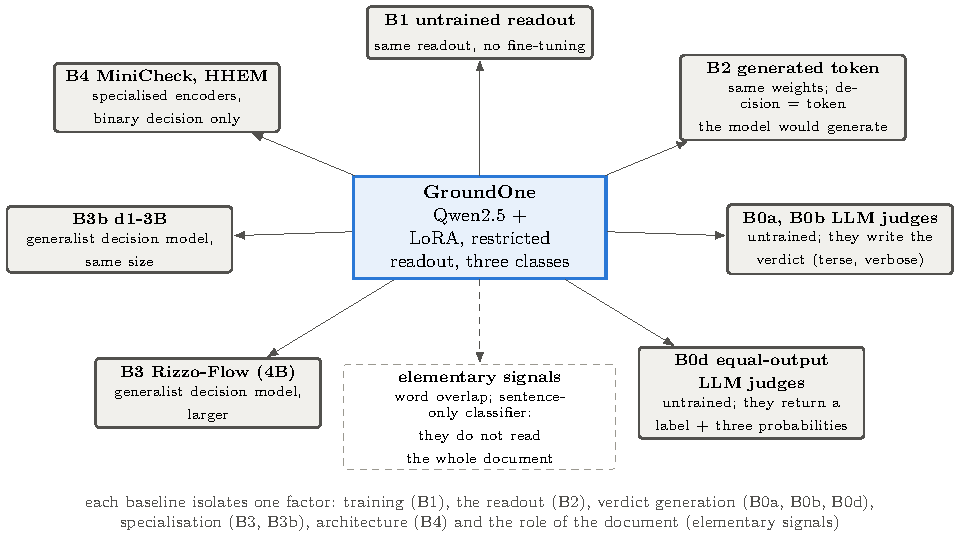
\includegraphics[width=\textwidth]{images/diagrams/setup_baseline_map_tikz.pdf}
\caption{Map of the baselines. Each one differs from GroundOne in one specific respect and therefore answers a different question: how much training matters (B1), how much the restricted readout matters compared with the generated token (B2), how much the way the verdict is produced matters (LLM judges B0a, B0b, B0d), how much specialisation matters compared with a general-purpose decision model (B3, B3b), how much the architecture matters (encoders B4) and how far one gets without reading the document (elementary cues).}
\label{fig:setup-baselines}
\end{figure}

\paragraph{Cues that never read the document as a whole.} Two elementary predictors set the minimum level that any
verifier must clear. The first scores a sentence by the share of its content words that also occur in the document. The
second is a bag-of-words classifier\footnote{A \emph{bag-of-words} classifier represents a text by the words, or the
short sequences of words, that it contains and by their frequencies, ignoring their order.} trained on the training
sentences alone, without the document. Both are described in Section~\ref{sec:data-eda}.

\paragraph{Untrained readout (B1).} The same Qwen2.5 models, without fine-tuning, are asked the three-way question for
each sentence, and the logits of the answer letters are read. An untrained model has no reason to interpret the
\texttt{Verdict:} marker as a question. This baseline therefore adopts the format with one explicit question per
sentence (Section~\ref{sec:method-readout}). In this way it measures what the decision-model mechanism offers before any
specialisation.

\paragraph{LLM judges (B0a, B0b).} The untrained models are also used in the way that is most common in
practice, that is, as LLM judges. They receive the document, the numbered answer and the list of sentences to check, and
they write a verdict for each sentence with greedy decoding\footnote{In \emph{greedy decoding} the model chooses the
most probable token at every step, without sampling: for the same input, the output is therefore always the same.}. The
\emph{terse} LLM judge produces one line ``\texttt{<number>: <letter>}'' per sentence. The \emph{verbose} LLM judge, instead,
writes a short justification for each sentence followed by the verdict. When a verdict cannot be parsed, a format
failure occurs: in the computation of accuracy it is counted as an error, and it is also reported separately.

\paragraph{Equal-output judges (B0d).} The terse and verbose LLM judges return less than GroundOne: one letter per sentence
and no probability. They therefore allow neither calibration, nor an adjustable threshold, nor the choice of a decision
policy. For this reason two further LLM judges are asked for exactly what GroundOne produces, namely a label and three
probabilities per sentence. The first writes the label and the probabilities in a JSON object, expressing the
probabilities as text: this is what a developer would obtain from the prompt alone. The second is the terse LLM judge, whose
three probabilities are read from the logits at the position of the letter it generates. It thus obtains the same
content at the cost of the terse LLM judge, and it is the strongest generative opponent. Both are calibrated with the same
transformation used for GroundOne, a temperature and a bias, fitted for each LLM judge on 200 answers of the dev set, so
that their probabilities receive the same treatment. The JSON prompt was chosen on twelve answers of the dev set, with
attention to format validity alone. The models copied verbatim a numeric example contained in the prompt, which was
therefore replaced by placeholders. Parsing is lenient, in the LLM judges' favour: the complete entries of a truncated
object are kept, and a missing label is derived from the probabilities. Decoding, finally, is not constrained by a
grammar~\cite{willard2023outlines}, so that the protocol remains that of the other LLM judges. This choice weighs mainly on
the format failures of the smallest model.

\paragraph{Readout versus generation (B2).} The fine-tuned GroundOne models are run with the same prompt and the same
single forward pass, but with a different decision rule. The verdict at each marker is not chosen among the three
letters alone, but is the token with the highest probability over the whole vocabulary, that is, the one that greedy
generation of a single token would produce. The three letters, with or without a leading space, correspond to the three
classes, and any other token is a format failure. This control leaves weights, prompt and cost unchanged and changes
only one aspect: whether or not the decision is restricted to the admissible options.

\paragraph{A general-purpose decision model: Rizzo-Flow (B3).} The open project Rizzo-Flow~\cite{rizzoflow} implements
the decision-model idea with a model of 4B parameters, fine-tuned on generic typed decisions. It runs in its own server,
based on llama.cpp~\cite{llamacpp}, and is queried over HTTP. The document and the numbered answer are passed to it as
shared state, that is, as a context common to all the questions, together with one three-way choice question for each
sentence. The model quantised to 4 bits is used, because the 8-bit one does not fit in memory alongside the operating
system.

\paragraph{A general-purpose decision model of the same size: d1-3B (B3b).} Liquid AI's d1-3B~\cite{liquid2026d1} is an
open decision model of 3.1B parameters, post-trained for typed decisions on a wide variety of tasks. It reads the
decision from restricted answer letters and shares the state across questions. It therefore belongs to the same readout
family as GroundOne and has the size of its larger model, but, unlike GroundOne, it is general-purpose. The comparison
with d1-3B thus isolates the value of specialisation with respect to a decision model that was already trained to
decide, rather than with respect to an untrained model. The model is run zero-shot with its own inference code, in
PyTorch on the GPU of the laptop and without network access. It receives the same state and the same questions as
Rizzo-Flow, with at most six questions per call on the same state. On LLM-AggreFact the documents longer than
1{,}500 tokens are split, for d1-3B as for GroundOne, into chunks of 1{,}500 tokens overlapping by 200, and for each
sentence the highest probability of support over the chunks is kept. A practical detail matters for reproducibility. On
the Apple GPU, PyTorch keeps the compiled kernels, that is, the programs executed by the GPU, for every new input
length, and never releases their memory. The evaluation therefore runs in worker processes that are restarted when the
memory occupied by the GPU driver exceeds 11\,GB; the restarts have no effect on the outputs.

\paragraph{Specialised encoders (B4).} MiniCheck-RoBERTa~\cite{tang2024minicheck} and HHEM-2.1-open~\cite{vectara2024hhem}
are the strongest small verifiers available today. They score each (document, sentence) pair independently and return a
single probability of support. As in MiniCheck, long documents are split into chunks of about 400 words, and for each
sentence the highest probability of support over the chunks is kept. The encoders have no three-way output, so they are
compared on the binary decision only. They run in PyTorch on the GPU of the laptop.

\paragraph{Published results.} For LLM-AggreFact, the scores of larger systems from the public leaderboard, such as
Qwen2.5-7B used zero-shot, are also reported. These scores are taken as published, without re-running the systems.

The slower systems are evaluated on subsamples of the test sets, mostly stratified\footnote{A subsample is
\emph{stratified} when it is drawn separately from each subgroup (stratum) of the original set, with a fixed number of
elements for each stratum, rather than from the whole set in a purely random way.}. Rizzo-Flow is evaluated on 300
answers of T1, 600 pairs of T3 and 1{,}100 items of T2, of which it scored 1{,}093, because seven exceeded its context.
The d1-3B model is evaluated on a random subsample of 4{,}000 items of T2, the untrained 3B on 600 answers of T1 and the
LLM judges on the 200 answers of the latency protocol described below. GroundOne and MiniCheck-RoBERTa are
instead evaluated on the complete test sets, as are, on T1 and T3, the untrained 0.5B, HHEM and d1-3B; the untrained 3B
is also evaluated on the whole of T3. Every comparison with a subsampled system is made on the items scored by both
systems.

\section{Metrics}
\label{sec:setup-metrics}

The share of hallucinated sentences differs between the dev set and T1 (Section~\ref{sec:data-eda}), so the primary
metrics are chosen so as not to depend on the base rate of the classes. For the three-way decision the main metric is
the balanced accuracy, that is, the mean recall over the three classes. Alongside it, the recall of each class and the
share of predictions assigned to each class are reported; the latter reveals a model that has collapsed onto a single
answer. For the binary decision two metrics are reported: the balanced accuracy at a threshold of 0.5, as in the
LLM-AggreFact leaderboard, and the AUROC of $P(\text{supported})$, which does not depend on any threshold. Calibration is
measured with the ECE defined in Section~\ref{sec:method-calibration}, with the Brier score and with the negative
log-likelihood. Selective prediction is measured with risk--coverage curves and with the AURC
(Section~\ref{sec:method-calibration})~\cite{geifman2017selective}. All metrics on T1 are also reported per task and per
band of $K$.

\section{Statistical protocol}
\label{sec:setup-statistics}

Every difference between two systems is accompanied by a 95\,\% confidence interval, obtained with a paired bootstrap
with $B = 2{,}000$ resamples~\cite{koehn2004significance,bergkirkpatrick2012significance,dror2018hitchhiker}. The
bootstrap recomputes the difference on many samples drawn with replacement from the test set, and the spread of the
values obtained measures its uncertainty. The resampling unit, however, is not the sentence but the group used in the
leakage check: the source document in RAGTruth, the document in LLM-AggreFact and the Wikipedia page in VitaminC. The
sentences of the same answer, and the answers about the same document, are in fact strongly correlated, and resampling
them independently would lead to intervals that are too narrow. On LLM-AggreFact the groups are resampled within each of
the eleven datasets, because the macro average gives every dataset the same weight. The bootstrap is \emph{paired}
because the two systems of a comparison are evaluated on the same resamples. The reported $p$-value is two-sided: it is
twice the share of resamples in which the difference has the opposite sign to the observed one, with a minimum of $1/B$,
where $B$ is the number of resamples. Figure~\ref{fig:setup-bootstrap} outlines the procedure.

\begin{figure}[htbp]
\centering
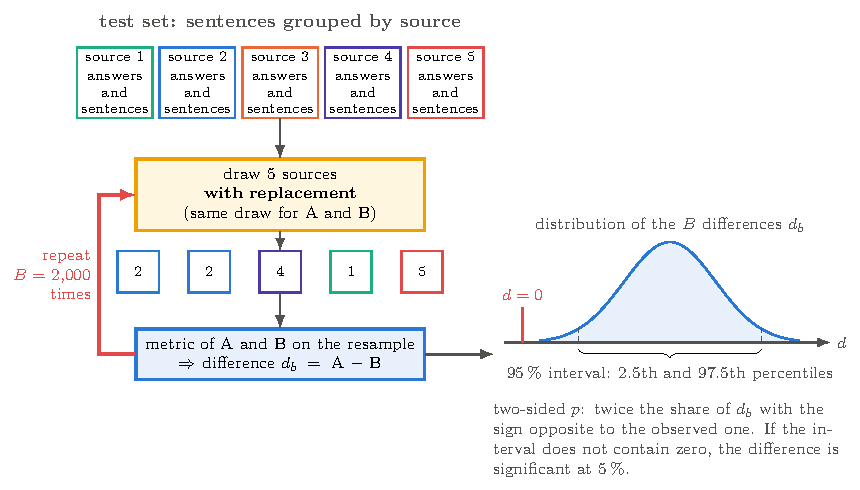
\includegraphics[width=\textwidth]{images/diagrams/setup_bootstrap_tikz.pdf}
\caption{Paired cluster bootstrap. The sentences of the test set are grouped by leakage group (source, document or page); at each repetition the groups are drawn with replacement, the metric of the two systems is computed on the same drawn sources and their difference is recorded. After $B = 2{,}000$ repetitions, the 2.5 and 97.5 percentiles of the differences give the 95\,\% interval, and the share of differences with the opposite sign to the observed one gives the $p$-value.}
\label{fig:setup-bootstrap}
\end{figure}

Two limits of the protocol must be stated in advance. The first is that about sixty comparisons are made without any
correction for multiple comparisons\footnote{When many statistical tests are carried out, the probability that some
differences turn out significant by pure chance increases. Corrections for multiple comparisons, such as the Bonferroni
correction, compensate for this effect by making the threshold of each test stricter.}. The conclusions therefore rest
on intervals that lie well away from zero, and no difference with a $p$-value close to 0.05 is considered established.
The second is that resampling the data does not capture the variability due to training, which the two runs of the 0.5B
document separately (Section~\ref{sec:results-seeds}).

\section{Latency, energy and hardware}
\label{sec:setup-protocol}

Latency is measured on 200 answers of T1, 50 from each band of $K$, so that long answers are as well represented as
short ones. GroundOne, the readout with one question per sentence and all the LLM judges run in process on MLX,
that is, inside the same process that invokes them, and they verify one answer at a time, as a verifier integrated in a
local assistant would. The first three answers serve as warm-up and are excluded from the measurement. For GroundOne and
for the readout with one question per sentence, each answer is timed three times and the median is kept. The generative
LLM judges, instead, are timed only once, because greedy decoding is deterministic and each run lasts much longer. The
reported time is the wall-clock time of the model call for one answer, from which the time per decision is derived. Chapter~\ref{sec:results} repeats this measurement, on the same answers, in three variants described where their results are reported (Section~\ref{sec:results-latency-split}): with the reading of the text separated from the decision, with part of the prompt already in the KV cache, the same for GroundOne and for the LLM judges, and with one sentence of the answer changed after a first verification. The read-ahead of the application is measured in Swift on the same answers (Section~\ref{sec:studio-flow}).

Times were also recorded for the encoders, for Rizzo-Flow and for d1-3B, but under conditions that do not allow a fair
comparison. The encoders ran in PyTorch and scored each sentence separately, re-reading the document every time, which
penalises them. Rizzo-Flow ran in a different inference engine, with 4-bit weights and behind an HTTP interface. The
d1-3B model, finally, ran in PyTorch with its own code and with the worker restarts described above. For these systems,
therefore, no conclusion about latency is drawn.

Energy is measured with \texttt{powermetrics}, the macOS tool that reports every 200 milliseconds the power drawn by the
CPU, the GPU and the Neural Engine, the NPU of Apple processors. For each system, the idle power with the model already
loaded is first measured for 60 seconds. Then 100 answers of the latency subset, 25 per band of $K$, are verified once.
The energy of a verification is the mean power during the run, net of the idle power, multiplied by the duration of the
run and divided by the number of answers. The measurement covers the computing units of the chip, but not the memory,
the display or the storage. It was taken at night, with the machine otherwise idle, and only without a cache.

Three measurements concern locality directly. The first checks independence from the network: a complete evaluation of
T1 is repeated with the libraries in offline mode and inside a macOS sandbox that denies the process any network access,
and its predictions are compared with those of the original run. The second measures the effect of quantisation: the
same adapter of the 0.5B model is applied to the original 16-bit (bf16) weights and evaluated on T1 and T3. The third
measures co-residence: a single process loads the generator of the demonstration application
(Chapter~\ref{ch:studio}), Qwen2.5-3B-Instruct quantised to 4 bits, and a GroundOne verifier; for 30 documents of T1, ten
per task, the generator writes an answer of at most 300 tokens and GroundOne verifies it. The peak memory allocated by
MLX and the generation and verification times are recorded. The document is given directly, as in RAGTruth, so the
retriever is not included. These measurements, too, run entirely inside the network-denying sandbox.

In every experiment only one model runs at a time, and a memory guard watches every long job, recording the free memory
and the swap throughout its duration. Results are written once and never overwritten, and each run stores its own
configuration. In this way every number in Chapter~\ref{sec:results} can be traced back to the run that produced it.

\section{Licences and terms of use}
\label{sec:setup-licences}

The independence that the thesis pursues also concerns the legal level: a local verifier is of little use if one of its
components can be used only through an external service or under a paid licence. Table~\ref{tab:setup-licences} reports
the licence of every model, dataset and software component used in the thesis, verified on the official page of each.

\begin{table}[htbp]
\centering
\caption{Licences of the components used in the thesis, verified on the official pages on 22 October 2026. The
quantised versions in MLX format inherit the licence of the original model.}
\label{tab:setup-licences}
\small
\begin{tabularx}{\textwidth}{@{}>{\raggedright\arraybackslash}p{0.34\textwidth}>{\raggedright\arraybackslash}p{0.2\textwidth}>{\raggedright\arraybackslash}X@{}}
\toprule
Component and role & Licence & Relevant conditions \\
\midrule
\multicolumn{3}{@{}l}{\textit{Models}} \\
Qwen2.5-0.5B-Instruct: base of GroundOne 0.5B & Apache 2.0 & Free use, including commercial use, with attribution. \\ \addlinespace[2pt]
Qwen2.5-3B-Instruct: base of GroundOne 3B and generator of the application & Qwen Research License~\cite{qwen2024researchlicense} & Research and evaluation only; commercial use requires a licence from Alibaba Cloud. \\ \addlinespace[2pt]
MiniCheck-RoBERTa-Large (B4) & MIT & Free use. \\ \addlinespace[2pt]
HHEM-2.1-open (B4) & Apache 2.0 & Free use, with attribution. \\ \addlinespace[2pt]
Rizzo-Flow, Spark-X2.5 4B with LoRA (B3) & Apache 2.0 & Free use, with attribution. \\ \addlinespace[2pt]
d1-3B (B3b) & LFM Open License 1.0~\cite{liquid2025lfmlicense} & Commercial use permitted below 10 million dollars of annual revenue. \\ \addlinespace[2pt]
bge-small-en-v1.5: embedding model of the application & MIT & Free use. \\
\addlinespace
\multicolumn{3}{@{}l}{\textit{Data}} \\
RAGTruth annotations & MIT & The contexts come from MS~MARCO, restricted to non-commercial research~\cite{msmarco2026terms}, from news articles and from the Yelp Open Dataset, intended for educational use~\cite{yelpdataset}. \\ \addlinespace[2pt]
LLM-AggreFact & CC BY-ND 4.0 & The access condition allows its use as an evaluation benchmark and forbids its use for training~\cite{hf_llmaggrefact}. \\ \addlinespace[2pt]
VitaminC & CC BY-SA 3.0 & Sharing under the same licence. \\
\addlinespace
\multicolumn{3}{@{}l}{\textit{Software}} \\
MLX, mlx-lm, MLX Swift & MIT & Free use. \\ \addlinespace[2pt]
PySBD, llama.cpp & MIT & Free use. \\ \addlinespace[2pt]
PyTorch, Transformers, swift-transformers & BSD, Apache 2.0 & Free use. \\
\bottomrule
\end{tabularx}
\end{table}

Three consequences follow. The first is that all the components can be downloaded and run locally under licences that
permit their use for research, without depending on any remote service: the independence of the solution also holds at
the level of licences. The second concerns the reuse of the trained models. The adapter of GroundOne 0.5B applies to a
base released under the Apache 2.0 licence, whereas that of GroundOne 3B applies to a base with a research licence,
which restricts its use to research and evaluation; the same holds for the generator of the application of
Chapter~\ref{ch:studio}. A commercial deployment would therefore require the 0.5B model or a base with a permissive
licence. The third concerns the training data: the RAGTruth annotations are released under the MIT licence, but the
contexts on which they were written come in part from sources intended for non-commercial research or for educational
use. For this reason too, the trained adapters should be regarded as research artefacts; a legal assessment of their
commercial use is beyond the scope of this thesis. LLM-AggreFact, finally, is used only as a test set, in compliance
with its access condition (Section~\ref{sec:data-sources}).
